\begin{figure}[tbp]
\centering
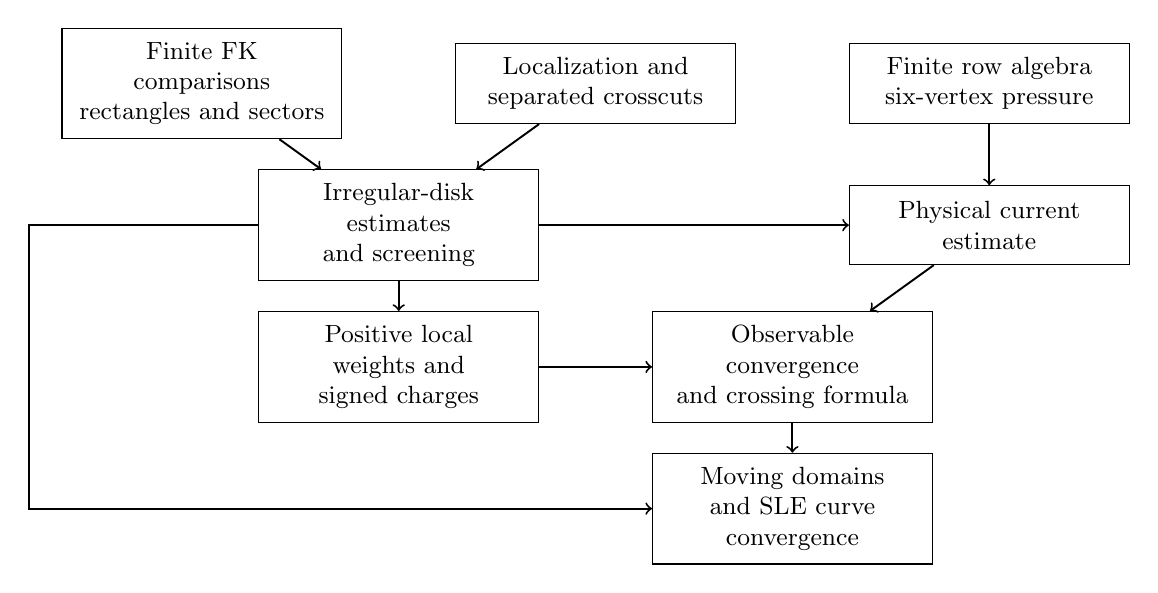
\begin{tikzpicture}[x=1cm,y=1cm,font=\small,
  block/.style={draw,align=center,text width=3.2cm,minimum height=1cm,inner sep=5pt},
  flow/.style={->,line width=.7pt}]
  \node[block] (finite) at (0,0) {Finite FK comparisons\\rectangles and sectors};
  \node[block] (local) at (5,0)
    {Localization and\\separated crosscuts};
  \node[block] (rows) at (10,0) {Finite row algebra\\six-vertex pressure};
  \node[block] (disks) at (2.5,-1.8) {Irregular-disk estimates\\and screening};
  \node[block] (current) at (10,-1.8) {Physical current\\estimate};
  \node[block] (charges) at (2.5,-3.6) {Positive local\\weights and\\signed charges};
  \node[block] (observable) at (7.5,-3.6) {Observable convergence\\and crossing formula};
  \node[block] (sle) at (7.5,-5.4) {Moving domains\\and SLE curve\\convergence};
  \draw[flow] (finite) -- (disks);
  \draw[flow] (local) -- (disks);
  \draw[flow] (rows) -- (current);
  \draw[flow] (disks) -- (current);
  \draw[flow] (disks) -- (charges);
  \draw[flow] (charges) -- (observable);
  \draw[flow] (current) -- (observable);
  \draw[flow] (observable) -- (sle);
  \draw[flow] (disks.west) -- (-2.2,-1.8) -- (-2.2,-5.4) -- (sle.west);
\end{tikzpicture}
\caption{The main proof dependencies. Localization in split tiled disks supplies the clear approaches and separated cuts needed to pass from finite network comparisons to actual-path decay. The disk estimates then feed both the local weight comparisons and the plane interpretation of the current. They also enter the moving-domain argument directly, through crossing estimates uniform over stopped exploration histories.}
\label{fig:dependencies}
\end{figure}
